
\documentclass[a4paper,12pt]{scrbook}
\usepackage{amsmath,amssymb,amsthm}
\usepackage{fancyvrb}
\usepackage{parskip}
\usepackage{lastpage}
\usepackage{verbatim,boxedminipage,enumitem}
\usepackage{ifthen}
\usepackage{color,graphicx}
\usepackage{pgf}
\usepackage{longtable}
\usepackage{upquote}
%\usepackage[all]{xy}
\usepackage{tobiShell}
\usepackage{tikz}
\usetikzlibrary{automata}
\usetikzlibrary{arrows}
\usepackage{pgf,pgfarrows,pgfnodes}
\usepackage{pgfplots}
\usepackage{circuitikz}
\usetikzlibrary{circuits}
\usetikzlibrary{circuits.logic.US}
\usepackage{mymath}
\usepackage{python}
%------------------------------------------------------------------
% Verbatim for console window - single line frame, no line numbers
%------------------------------------------------------------------
\DefineVerbatimEnvironment%
 {console}{Verbatim}
 {frame=single}

%--------------------------------------------------------
% Remove the vertical spacing before and after Verbatim.
%--------------------------------------------------------
\usepackage{atbeginend}
\BeforeBegin{console}{\mbox{}\\ \begin{minipage}{\textwidth}\vspace{3pt}}
\AfterEnd{console}{\vspace{4pt} \end{minipage} \\ }

\begin{document}
\thispagestyle{empty}

\begin{center}
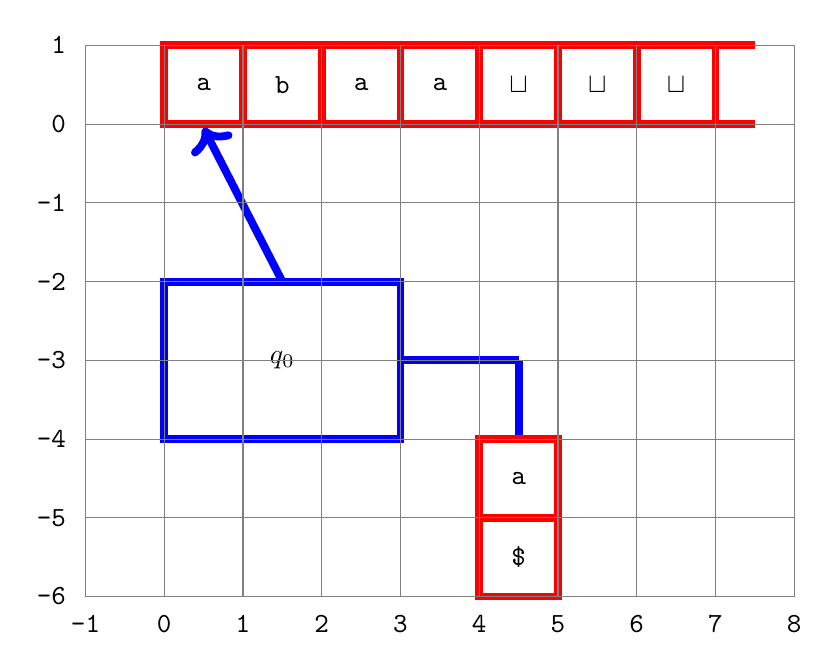
\begin{tikzpicture}

\draw (0.5, 0.5)
  node[draw, line width=0.1cm, , color=red,
       rounded corners=0cm, inner sep=0cm] {

\begin{minipage}[t][1.0cm]{1.0cm}
\mbox{}

\end{minipage}

};\draw (0.5, 0.5) node[color=black] {\texttt{a}};
\draw (1.5, 0.5)
  node[draw, line width=0.1cm, , color=red,
       rounded corners=0cm, inner sep=0cm] {

\begin{minipage}[t][1.0cm]{1.0cm}
\mbox{}

\end{minipage}

};\draw (1.5, 0.5) node[color=black] {\texttt{b}};
\draw (2.5, 0.5)
  node[draw, line width=0.1cm, , color=red,
       rounded corners=0cm, inner sep=0cm] {

\begin{minipage}[t][1.0cm]{1.0cm}
\mbox{}

\end{minipage}

};\draw (2.5, 0.5) node[color=black] {\texttt{a}};
\draw (3.5, 0.5)
  node[draw, line width=0.1cm, , color=red,
       rounded corners=0cm, inner sep=0cm] {

\begin{minipage}[t][1.0cm]{1.0cm}
\mbox{}

\end{minipage}

};\draw (3.5, 0.5) node[color=black] {\texttt{a}};
\draw (4.5, 0.5)
  node[draw, line width=0.1cm, , color=red,
       rounded corners=0cm, inner sep=0cm] {

\begin{minipage}[t][1.0cm]{1.0cm}
\mbox{}

\end{minipage}

};\draw (4.5, 0.5) node[color=black] {\texttt{$\sqcup$}};
\draw (5.5, 0.5)
  node[draw, line width=0.1cm, , color=red,
       rounded corners=0cm, inner sep=0cm] {

\begin{minipage}[t][1.0cm]{1.0cm}
\mbox{}

\end{minipage}

};\draw (5.5, 0.5) node[color=black] {\texttt{$\sqcup$}};
\draw (6.5, 0.5)
  node[draw, line width=0.1cm, , color=red,
       rounded corners=0cm, inner sep=0cm] {

\begin{minipage}[t][1.0cm]{1.0cm}
\mbox{}

\end{minipage}

};\draw (6.5, 0.5) node[color=black] {\texttt{$\sqcup$}};\draw[line width=0.1cm,red] (7.0,1.0) -- (7.5,1.0);
\draw[line width=0.1cm,red] (7.0,0.0) -- (7.5,0.0);

\draw (1.5, -3.0)
  node[draw, line width=0.1cm, , color=blue,
       rounded corners=0cm, inner sep=0cm] {

\begin{minipage}[t][2.0cm]{3.0cm}
\mbox{}

\end{minipage}

};\draw (1.5, -3.0) node[color=black] {$q_0$};\draw[line width=0.1cm,blue,->] (1.5,-2.0) -- (0.5,-0.05);

\draw (4.5, -4.5)
  node[draw, line width=0.1cm, , color=red,
       rounded corners=0cm, inner sep=0cm] {

\begin{minipage}[t][1.0cm]{1.0cm}
\mbox{}

\end{minipage}

};\draw (4.5, -4.5) node[color=black] {\texttt{a}};
\draw (4.5, -5.5)
  node[draw, line width=0.1cm, , color=red,
       rounded corners=0cm, inner sep=0cm] {

\begin{minipage}[t][1.0cm]{1.0cm}
\mbox{}

\end{minipage}

};\draw (4.5, -5.5) node[color=black] {\texttt{\$}};\draw[line width=0.1cm,blue] (3.0,-3.0) -- (4.5,-3.0);
\draw[line width=0.1cm,blue] (4.5,-3.0) -- (4.5,-3.95);
\draw[gray] (-1.0,-6.0) -- (-1.0,1);
\draw[gray] (0.0,-6.0) -- (0.0,1);
\draw[gray] (1.0,-6.0) -- (1.0,1);
\draw[gray] (2.0,-6.0) -- (2.0,1);
\draw[gray] (3.0,-6.0) -- (3.0,1);
\draw[gray] (4.0,-6.0) -- (4.0,1);
\draw[gray] (5.0,-6.0) -- (5.0,1);
\draw[gray] (6.0,-6.0) -- (6.0,1);
\draw[gray] (7.0,-6.0) -- (7.0,1);
\draw[gray] (8.0,-6.0) -- (8.0,1);
\draw[gray] (-1.0,-6.0) -- (8,-6.0);
\draw[gray] (-1.0,-5.0) -- (8,-5.0);
\draw[gray] (-1.0,-4.0) -- (8,-4.0);
\draw[gray] (-1.0,-3.0) -- (8,-3.0);
\draw[gray] (-1.0,-2.0) -- (8,-2.0);
\draw[gray] (-1.0,-1.0) -- (8,-1.0);
\draw[gray] (-1.0,0.0) -- (8,0.0);
\draw[gray] (-1.0,1.0) -- (8,1.0);
\draw(-1, -6) node [font=\ttfamily, label=below:{\texttt{-1}}] {};
\draw(0, -6) node [font=\ttfamily, label=below:{\texttt{0}}] {};
\draw(1, -6) node [font=\ttfamily, label=below:{\texttt{1}}] {};
\draw(2, -6) node [font=\ttfamily, label=below:{\texttt{2}}] {};
\draw(3, -6) node [font=\ttfamily, label=below:{\texttt{3}}] {};
\draw(4, -6) node [font=\ttfamily, label=below:{\texttt{4}}] {};
\draw(5, -6) node [font=\ttfamily, label=below:{\texttt{5}}] {};
\draw(6, -6) node [font=\ttfamily, label=below:{\texttt{6}}] {};
\draw(7, -6) node [font=\ttfamily, label=below:{\texttt{7}}] {};
\draw(8, -6) node [font=\ttfamily, label=below:{\texttt{8}}] {};
\draw(-1, -6) node [font=\ttfamily, label=left:{\texttt{-6}}] {};
\draw(-1, -5) node [font=\ttfamily, label=left:{\texttt{-5}}] {};
\draw(-1, -4) node [font=\ttfamily, label=left:{\texttt{-4}}] {};
\draw(-1, -3) node [font=\ttfamily, label=left:{\texttt{-3}}] {};
\draw(-1, -2) node [font=\ttfamily, label=left:{\texttt{-2}}] {};
\draw(-1, -1) node [font=\ttfamily, label=left:{\texttt{-1}}] {};
\draw(-1, 0) node [font=\ttfamily, label=left:{\texttt{0}}] {};
\draw(-1, 1) node [font=\ttfamily, label=left:{\texttt{1}}] {};
\end{tikzpicture}

\end{center}

\end{document}
